\chapter{\projectname-\LaTeX{}模板快速入门}\label{chap:latex-quickstart}

为方便使用及更好地展示\LaTeX{}排版的优秀特性,\projectname 的框架和文件体系进行了细致地处理,尽可能地对各个功能和板块进行了模块化封装,对于初学者来说,众多的文件目录也许一开始让人觉得有些无所适从,但阅读完下面的使用说明后,会发现原来使用思路是简单而清晰的,而且,当对\LaTeX{}有一定的认识和了解后,会发现其相对Word类排版系统极具吸引力的优秀特性。所以,如果是初学者,请不要退缩,请稍加尝试和坚持,以领略到\LaTeX{}的非凡魅力,并可以通过阅读相关资料如\LaTeX{} Wikibook \cite{wikibook2014latex} 来完善自己的使用知识。

\section{先试试效果}
\begin{figure}[!hptb]
        \centering
        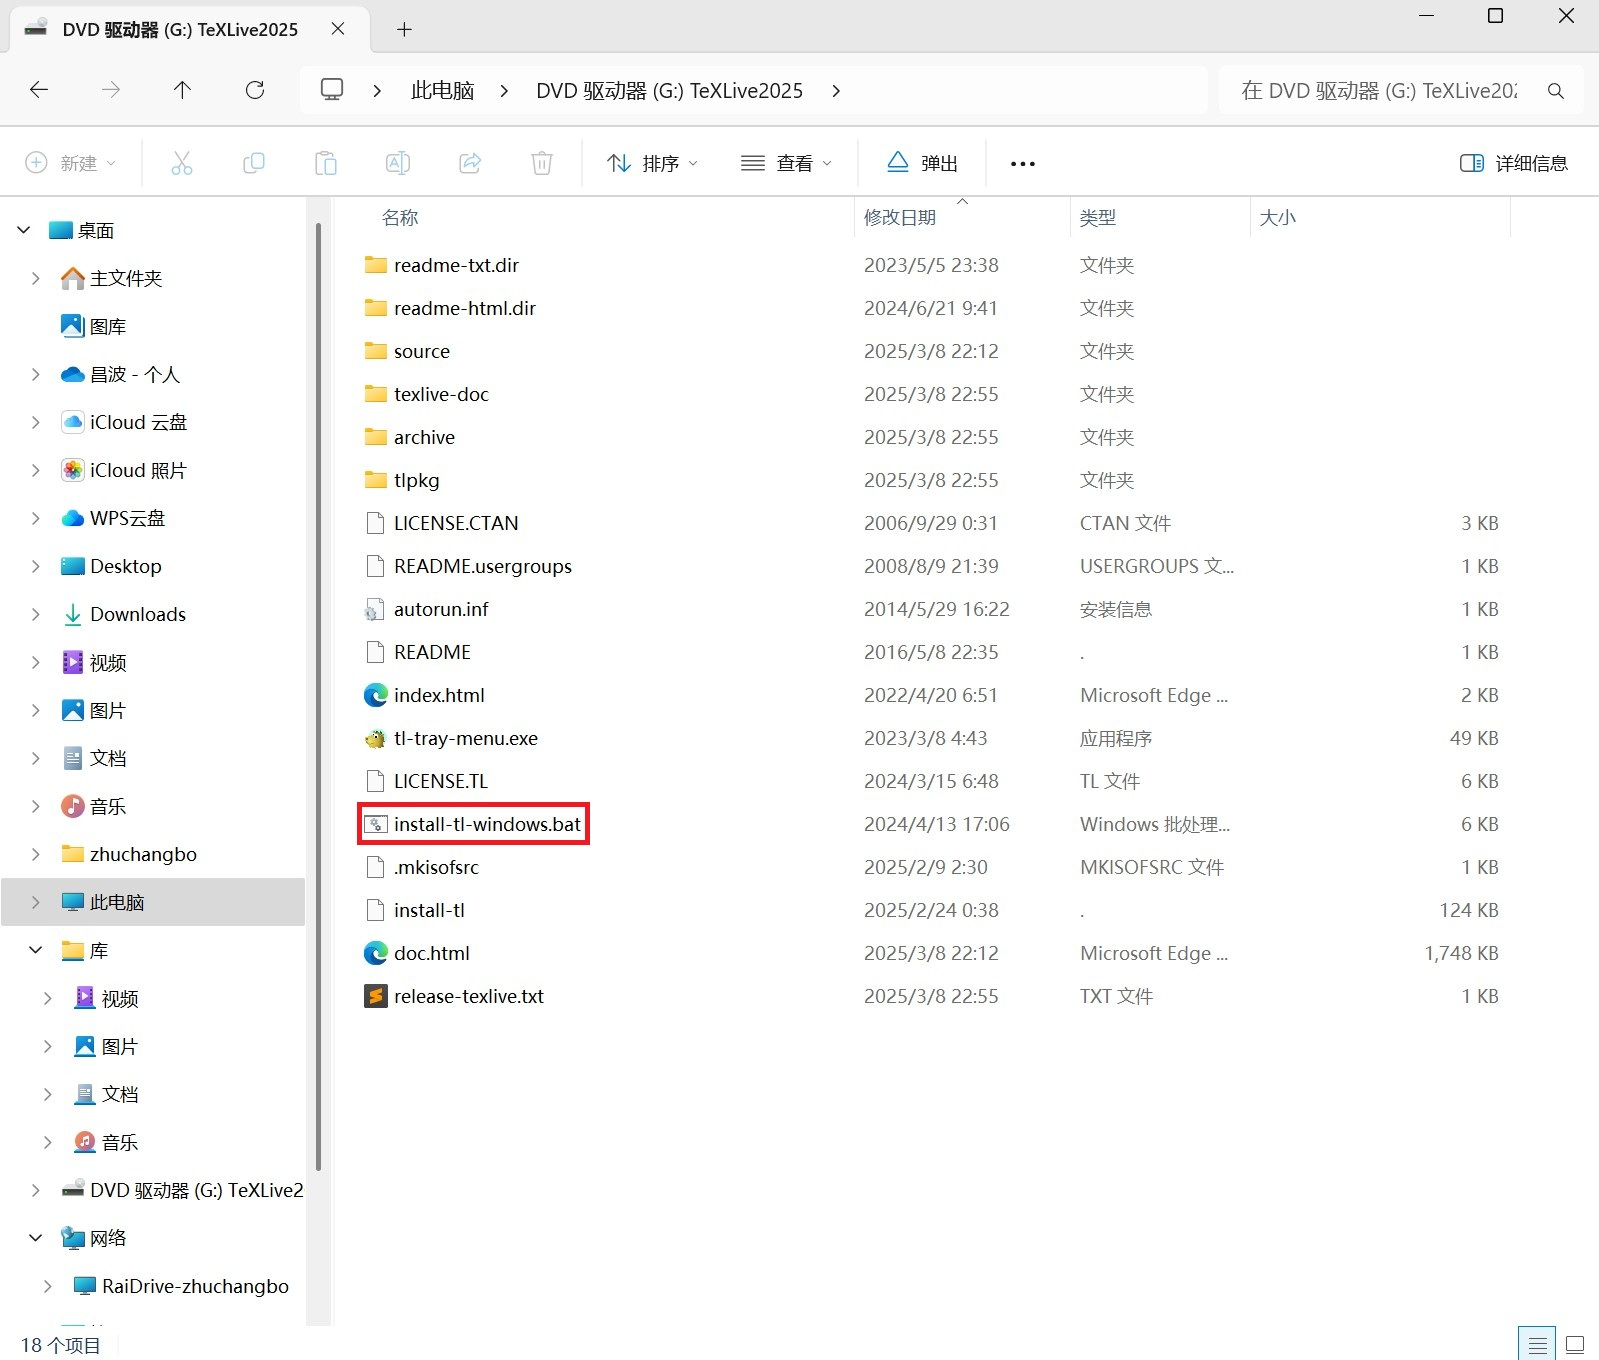
\includegraphics[width=0.8\textwidth]{doc/figures/texlive-iso-content.jpg}
        \caption{\TeX~Live-2025目录}
        \label{fig:texlive-iso-content}
        \end{figure}
\begin{enumerate}
    \item \emph{安装软件}:
        根据所用操作系统和章节~\ref{sec:system}中的信息安装\LaTeX{}编译环境。下面基于windows 11演示安装\TeX~Live和vscode/TeXstudio。\TeX~Live的详细安装教程参见:\href{https://texdoc.org/serve/texlive-zh-cn.pdf/0}{texlive-zh-cn.pdf}(\url{https://texdoc.org/serve/texlive-zh-cn.pdf/0})或者\href{https://github.com/OsbertWang/install-latex-guide-zh-cn}{install-latex-guide-zh-cn}(https://github.com/OsbertWang/install-latex-guide-zh-cn)。
        

        第一步,下载\TeX~Live的ISO镜像文件。国内比较方便的下载站点有 \href{https://mirrors.tuna.tsinghua.edu.cn}{清华大学tuna镜像站}(\href{https://mirrors.tuna.tsinghua.edu.cn/CTAN/systems/texlive/Images/texlive.iso}{点击下载texlive.iso})、\href{https://mirror.nju.edu.cn}{南京大学开源镜像站}(\href{https://mirror.nju.edu.cn/CTAN/systems/texlive/Images/texlive.iso}{点击下载texlive.iso})、\href{https://mirrors.ustc.edu.cn}{中科大开源镜像站}(\href{https://mirrors.ustc.edu.cn/CTAN/systems/texlive/Images/texlive.iso}{点击下载texlive.iso})等等。下载完成后,如图\ref{fig:texlive-iso-content},直接点击下载的文件“texlive.iso”,进入texlive目录。
        

        第二步,以管理员身份运行图\ref{fig:texlive-iso-content}中的批处理文件“install-tl-windows.bat”(shell脚本install-tl是包括Linux系统在内的类unix系统运行的安装文件),在弹出的如图\ref{fig:texlive-tl-gui}所示界面中点击左下角“Advanced(高级)”按钮,可进行相关参数配置。
        \begin{figure}[!hptb]
        \centering
        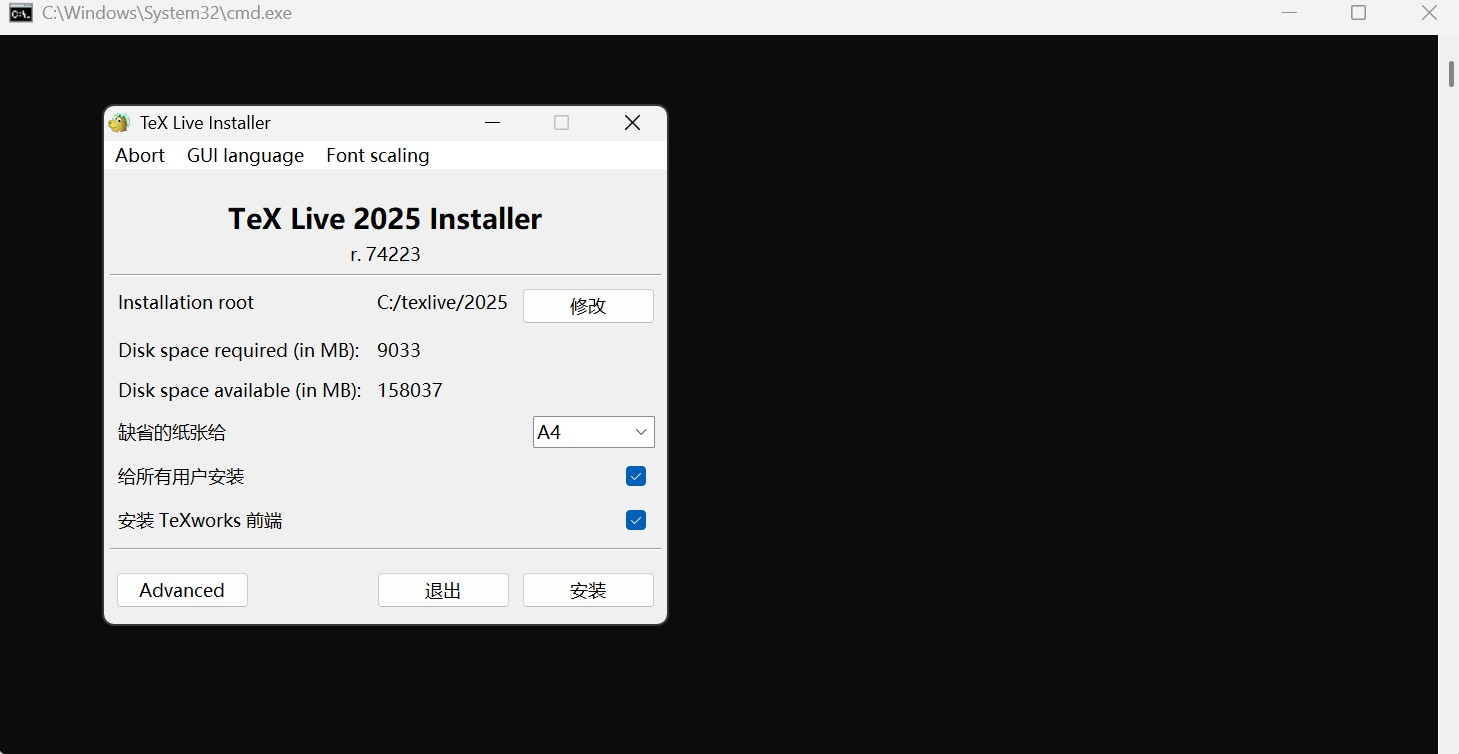
\includegraphics[width=0.8\textwidth]{doc/figures/texlive-tl-gui.jpg}
        \caption{\TeX~Live-2025安装界面}
        \label{fig:texlive-tl-gui}
        \end{figure}

        第三步,如图\ref{fig:texlive-tl-gui-adv},指定三个TDS树目录:
        \begin{itemize}
            \item TEXDIR: 安装根目录,指定TEXMFMAIN树所在目录,例如“C:/texlive”;
            \item TEXMFLOCAL: 指定TEXMFLOCAL树所在目录,系统管理员用来安装供整个系统使用的额外的或更新过的宏包、字体等的目录树,以避免TeX 系统升级等原因而受到影响;
            \item TEXMFHOME: 用户用来安装供他们自己独立使用的的额外的或更新过的宏包、字体等的目录树。这个变量根据不同的用户选择不同的个人目录,例如“\~/texmf”。
        \end{itemize}
        其它选项一般保持默认配置即可。
        \begin{figure}[!hptb]
        \centering
        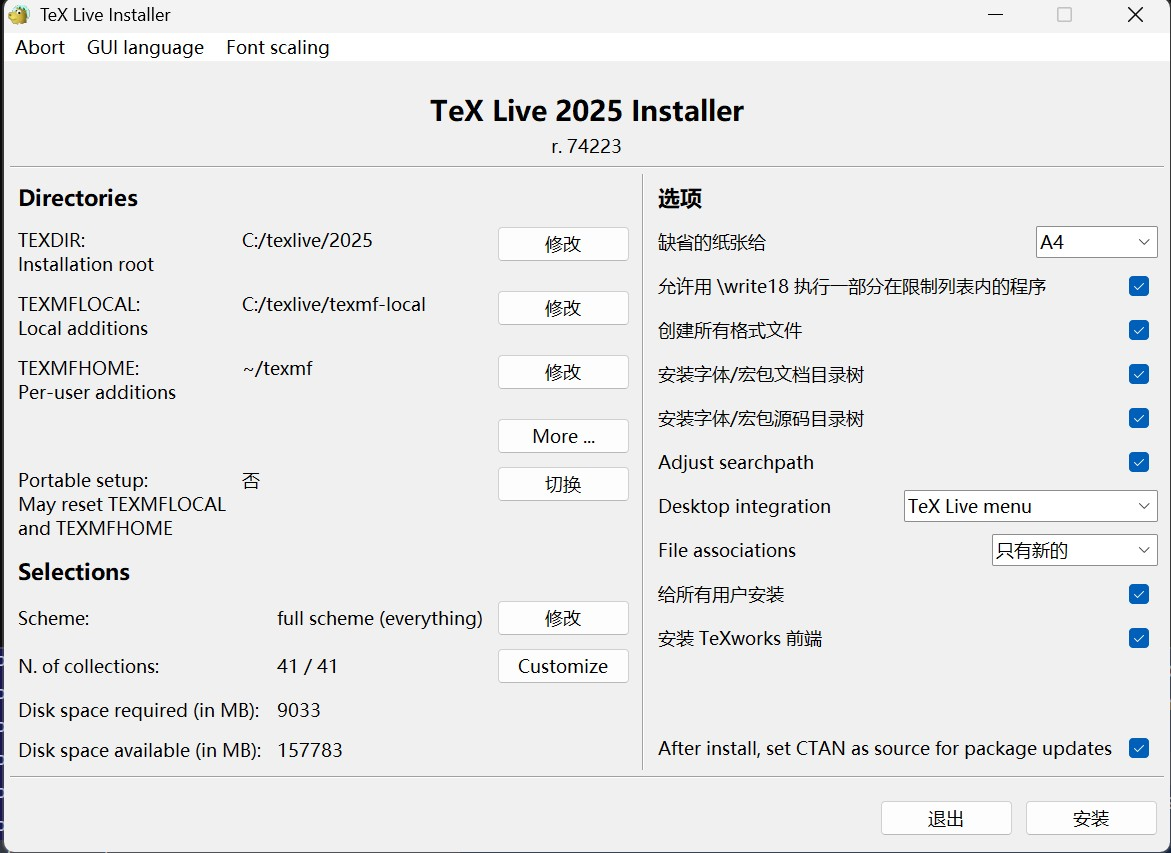
\includegraphics[width=0.8\textwidth]{doc/figures/texlive-tl-gui-adv.jpg}
        \caption{\TeX~Live-2025高级配置界面}
        \label{fig:texlive-tl-gui-adv}
        \end{figure}
        
        第四步,点击图\ref{fig:texlive-tl-gui-adv}右下角所示的“安装”按钮开始安装。直到安装完成,点击“完成”即可。

        第五步,安装TeXstudio。首先\href{https://mirrors.tuna.tsinghua.edu.cn/github-release/texstudio-org/texstudio/LatestRelease/texstudio-4.8.8-win-qt6-signed.exe}{下载TeXstudio},然后,点击“texstudio-4.8.8-win-qt6-signed.exe”进行安装即可。也可以通过\href{https://texstudio.sourceforge.net/}{texstudio官网}(\url{https://texstudio.sourceforge.net/})下载最新版本安装。

        第六步,安装vscode。首先\href{https://vscode.download.prss.microsoft.com/dbazure/download/stable/488a1f239235055e34e673291fb8d8c810886f81/VSCodeUserSetup-x64-1.102.3.exe}{下载vscode},也可以访问\href{https://code.visualstudio.com/Download}{vscode网站}(\url{https://code.visualstudio.com/Download})下载最新版本。然后点击下载的文件进行安装。

    \item \emph{获取模板}:
        下载 \href{https://github.com/changbozhu/\projectname}{\projectname} 模板并解压。 \projectname 模板不仅提供了相应的类文件,同时也提供了包括参考文献等在内的完成中文论文的一切要素,所以,下载时,推荐下载整个 \projectname 模版文件夹,而不是单独的文档类。

        当然,也可以通过git命令克隆仓库到本地: 
        
        \texttt{git clone https://github.com/changbozhu/\projectname.git}
       
    
    \item \emph{基于TeXstudio编译文档}:
        TeXstudio是集成度较高的\LaTeX{}开发编辑器。本部分简单介绍TeXstudio编译本模版的方法。
        
        第一步,打开TeXstudio,在菜单栏打开“选项”->“设置TeXstudio”。如图\ref{fig:texstudio-setup}所示,把“默认编译器”调整为“PdfLaTeX”,“默认文献工具”调整为“Biber”。然后选择右下角的“确定”。
        \begin{figure}[!hptb]
            \centering
            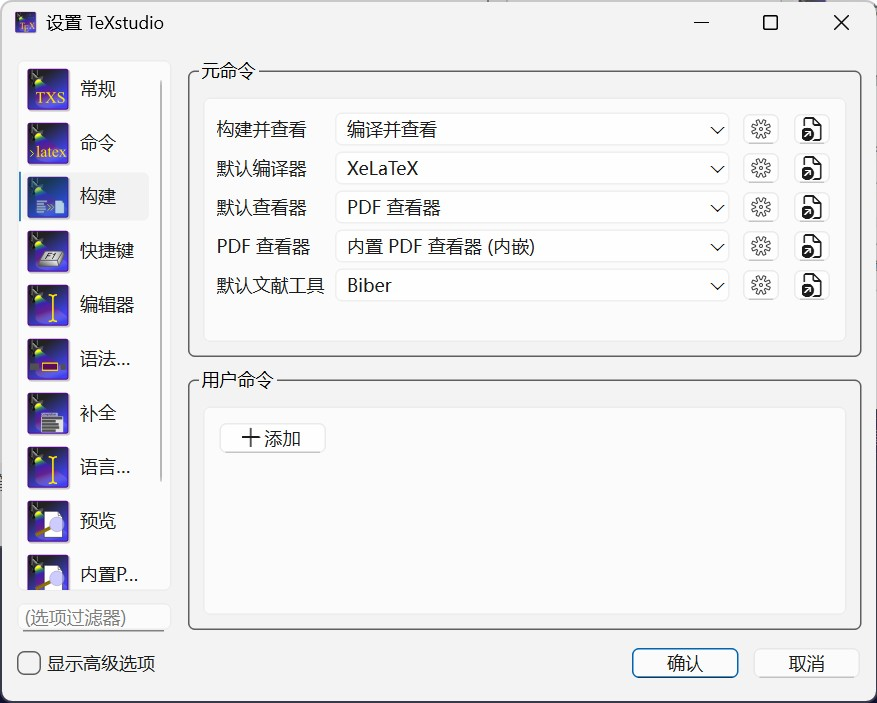
\includegraphics[width=0.6\textwidth]{doc/figures/texstudio-setup.jpg}
            \caption{TeXstudio设置界面}
            \label{fig:texstudio-setup}
        \end{figure}

        第二步,在TeXstudio菜单中打开“文件”->“打开”,出现文件浏览器后导航到模版目录,选择并打开文件“\projectname.tex”,如图\ref{fig:texstudio-doc}所示。
        \begin{figure}[!hptb]
            \centering
            \includegraphics[width=0.6\textwidth]{doc/figures/texstudio-\projectname.jpg}
            \caption{TeXstudio打开文档并构建}
            \label{fig:texstudio-doc}
        \end{figure}

        第三步,如图\ref{fig:texstudio-doc}所示,点击红色框内的绿色按钮,构建并查看文档。
    
    \item \emph{基于vscode编译文档}:
    
 		第一步,打开vscode,如图\ref{fig:vscode-ext}所示,点击左侧栏的“扩展”(如图所示的红色框区域),在图所示的蓝色框搜索区域搜索“Chinese”,在搜索结果中选择“Chinese (Simplified) Language Pack for Visual Studio Code”插件安装。接着搜索“latex workshop”,选择第一个LaTeX Workshop插件进行安装。安装完成后重启vscode。
 		\begin{figure}[!hptb]
            \centering
            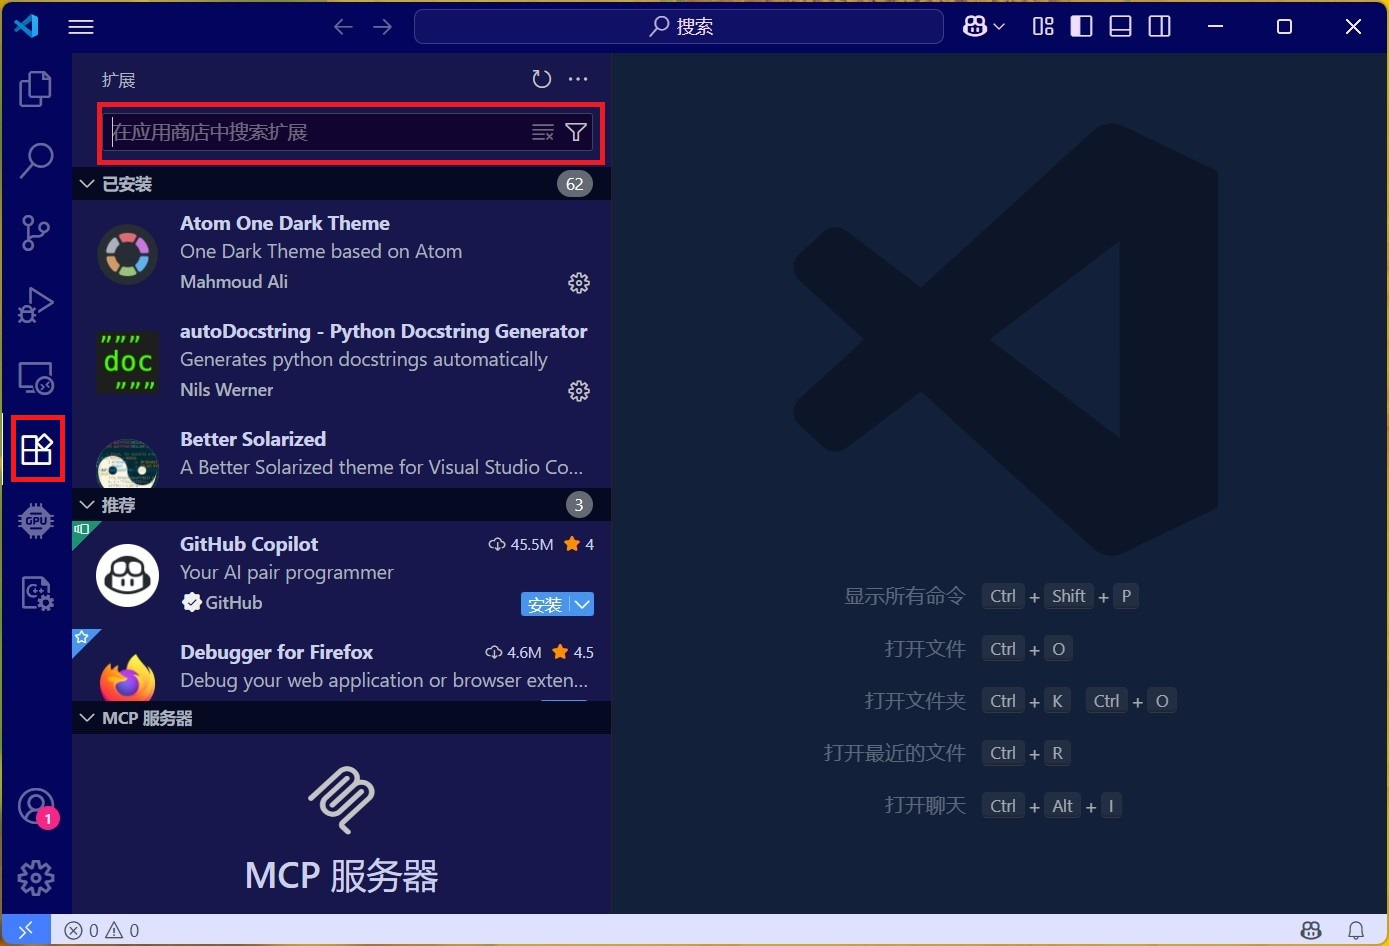
\includegraphics[width=0.8\textwidth]{doc/figures/vscode-ext.jpg}
            \caption{vscode安装插件}
            \label{fig:vscode-ext}
        \end{figure}

 		第二步,点击菜单栏“文件”->“打开文件夹”,在弹出的浏览器窗口选择模版所在文件夹并打开。如图\ref{fig:vscode-openfile}所示,选择左侧边栏最上边的的“资源管理器",可以查看模版文件夹内全部文件,打开”\projectname.tex“,左侧边栏出现”\TeX“字样按钮,点击这个”\TeX“字样按钮。
        \begin{figure}[!hptb]
            \centering
            \includegraphics[width=0.8\textwidth]{doc/figures/vscode-open\projectname.jpg}
            \caption{在vscode中打开文档}
            \label{fig:vscode-openfile}
        \end{figure}

        第三步,展开“构建LaTeX项目”,如图\ref{fig:vscode-buildfile}所示。点击“配方:xelatex->biber->xelatex->xelatex”编译生成文档。
        \begin{figure}[!hptb]
            \centering
            \includegraphics[width=0.8\textwidth]{doc/figures/vscode-build\projectname.jpg}
            \caption{在vscode构建文档}
            \label{fig:vscode-buildfile}
        \end{figure}

        第四步,如图\ref{fig:vscode-pdfview}所示,点击“查看LaTeX PDF”。
 		\begin{figure}[!hptb]
            \centering
            \includegraphics[width=0.8\textwidth]{doc/figures/vscode-\projectname-pdf.jpg}
            \caption{在vscode查看文档}
            \label{fig:vscode-pdfview}
        \end{figure}
 		

    \item \emph{基于命令行编译文档}:
        \begin{enumerate}
            \item Windows:双击运行builder.bat脚本。
            \item Linux或MacOS: {\scriptsize \verb|terminal| -> \verb|chmod +x ./builder.sh| -> \verb|./builder.sh xa \projectname|}
            \item 任意系统:都可使用\LaTeX{}编辑器打开 \projectname.tex文件并选择xelatex编译引擎进行编译。
        \end{enumerate}
    \item \emph{错误处理}:若编译中遇到了问题,请先查看“常见问题”(章节~\ref{sec:qa})。
\end{enumerate}

编译完成即可获得本PDF说明文档。而这也完成了学习使用 \projectname 撰写论文/书籍/报告的一半进程。什么?这就学成一半了,这么简单???,是的,就这么简单!

\section{文档目录简介}

\subsection{文档根目录}

\projectname.tex为主文档文件,默认是本模板的说明文档主文件,也作为样例供用户参考。\projectname.tex供用户定义自己的论文。主文档设计和规划了论文的整体框架,通过对其阅读可以了解整个论文框架的搭建。


\begin{enumerate}
    \item \projectname.tex: 主文件样例,用户文档主文件。
    \item ref.bib:参考文献信息库。
    \item builder.sh: linux/macos下的shell编译脚本。
    \item builder.bat: windows下的dos编译脚本。
    \item usercustom.sty: 用户自定义命令接口。
\end{enumerate}

\subsection{编译脚本}

\begin{itemize}
    \item Windows:双击Dos脚本builder.bat可得全编译后的PDF文档,其存在是为了帮助不了解\LaTeX{}编译过程的初学者跨过编译这第一道坎,请勿通过邮件传播和接收此脚本,以防范Dos脚本的潜在风险。
    \item Linux或MacOS:在terminal中运行
        \begin{itemize}
            \item \verb|./builder.sh xa <mainfilename>|:获得全编译后的PDF文档
            \item \verb|./builder.sh x <mainfilename>|:快速编译,不会生成文献引用
        \end{itemize}
\end{itemize}

全编译指运行 \verb|xelatex+bibtex+xelatex+xelatex| 以正确生成所有的引用链接,如目录,参考文献及引用等。在写作过程中若无添加新的引用,则可用快速编译,即只运行一遍\LaTeX{}编译引擎以减少编译时间。

\subsection{Tmp文件夹}

运行编译脚本后,编译所生成的文档皆存于Tmp文件夹内,包括编译得到的PDF文档,其存在是为了保持工作空间的整洁,因为好的心情是很重要的。

\subsection{style文件夹}

包含ntuthesis文档类的定义文件和配置文件,GB/T 7714引用样式,通过对它们的修改可以实现特定的模版设定。

\begin{enumerate}
    \item \projectname.cls:文档类定义文件,论文的最核心的格式即通过它来定义的。
    \item \projectname.cfg:文档类配置文件,设定如目录显示为“目~录”而非“目录”。
    \item cnbasesetup.sty:常用宏包及文档设定,如字体族、参考文献样式、文献引用样式等。
    \item \projectname setup.sty:设置文档类中一些命令、环境、页眉页脚等”。
\end{enumerate}

\subsection{mlstyle文件夹}
包含用户自定义的机器学习样式文件,如数学样式、神经网络绘图样式、贝叶斯智能体绘图样式等。
\begin{enumerate}
    \item mlmath.sty: 定义了数学基本符号规范,加强了机器学习相关的数学表达式。
    \item bayesianagent.sty: 定义了贝叶斯智能体的一些绘图命令。
    \item deeplearningplot.sty: 定义了深度学习的一些绘图命令,待开发。
    \item snnplot.sty: 定义了脉冲神经网络的一些绘图命令,待开发。
\end{enumerate}

\subsection{doc文件夹}
文件夹内为用户文档的所有实体内容,正常情况下,用户无需修改本文件夹。


\subsection{figures文件夹}
文件夹位默认图片存放与搜索位置,用户可将图片存放于此位置,支持格式有:.jpg, .png, .pdf。不建议为各章节图片建子目录,即使图片众多,若命名规则合理,图片查询亦是十分方便。

\subsection{ \projectname 文件夹}
文档几个模块的基本信息,如论文信息、主内容信息、附录信息等 \footnote{对于研究生学位论文,此文件夹为 \projectname;对于本科生学位论文,此文件夹为 ntudesign 文件夹。}。
\begin{itemize}
    \item FrontBookinfo.tex:为论文信息。
    \item Frontmatter.tex:为论文前序内容。
    \item Mainmatter.tex:列出需要出现的Chapter。写论文时,可以只列出当前章节,以快速编译查看,当论文完成后,再对所有章节进行索引即可。
    \item Appendix.tex:为附录内容。
    \item Backmatter.tex:为论文作者简介和致谢部分等。
\end{itemize}

\subsection{chapters文件夹}
文件夹内为论文的所有实体内容,正常情况下,这也是\textbf{使用 \projectname 撰写论文/书籍/报告时,主要关注和修改的一个位置,注:所有文件都必须采用UTF-8编码,否则编译后将出现乱码文本},\textbf{添加新章时,可拷贝一个已有的章文件再重命名,以继承文档的 UTF8 编码}。

\section{引入 \projectname 文档类}
在文档开始,通过下列命令引入 \projectname.cls文档类
\begin{lstlisting}[language=tex]
    \documentclass[doctor,academic]{style/ntuthesis}%
\end{lstlisting}

